\chapter{セルフトリガを用いた応答評価試験}
この章では,セルフトリガを用いた粒子線に対する応答評価試験について述べる.\ref{sec:latency}節で粒子線を用いた応答評価試験のために必要だったLatencyチューニング機能について述べ,そのあとに,\ref{sec:selfsetup}節で評価試験セットアップ,\ref{sec:selfhow}節で手順,\ref{sec:selfconc}節で取得データの結果を示し,\ref{sec:selfsum}節で考察を行なっている.

\section{Latencyチューニング機能の追加}
\label{sec:latency}
この節では,粒子線に対する応答評価のために必要だったLatencyチューニング機能について述べる.
\subsection{YARRにおけるトリガDAQとLatencyの意義}
YARRソフトウェアを用いたデータ取得におけるトリガDAQについて説明する図を図\ref{fig:YARRDAQ}に示す\par
\begin{figure}[h]
  \centering
  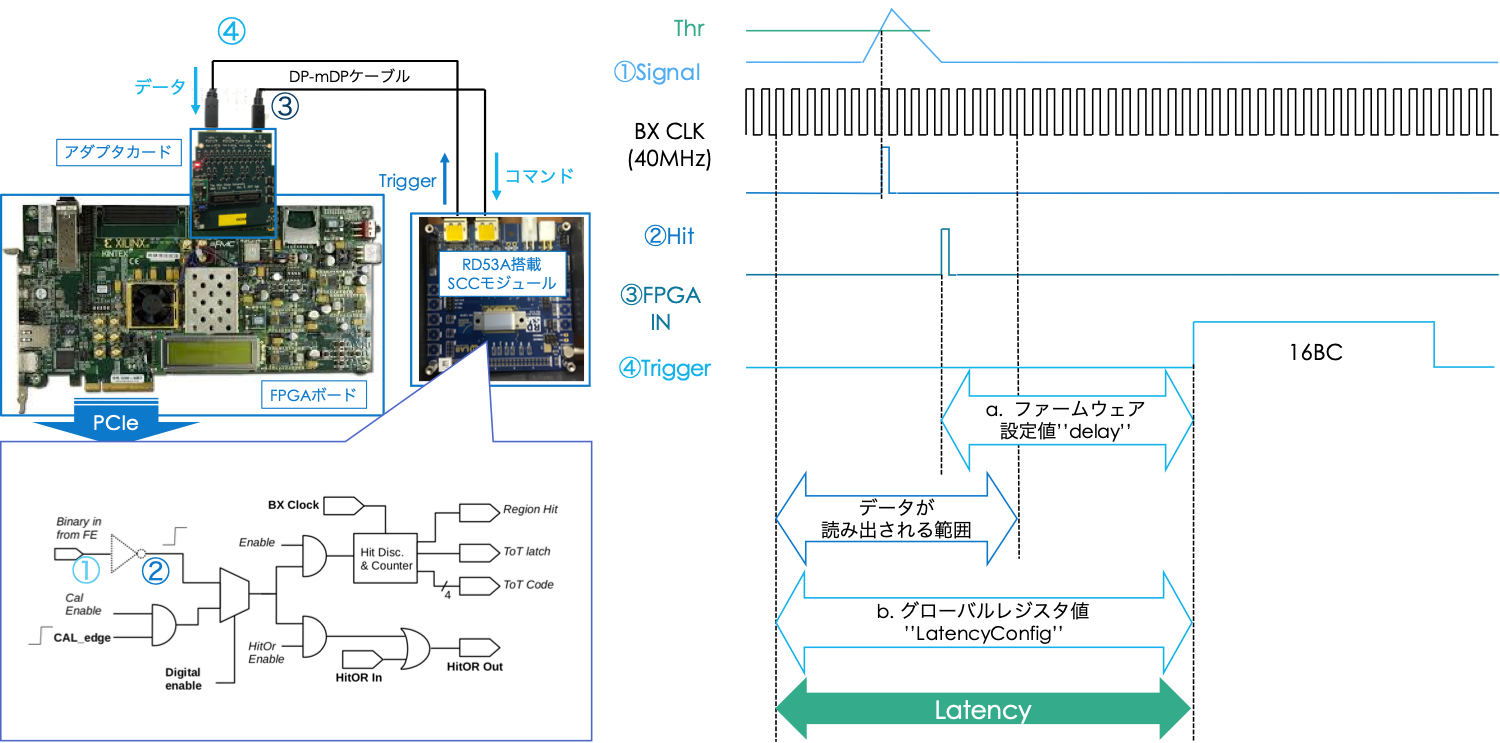
\includegraphics[width=16cm]{./figure/DAQ_sigfig.png}
  \caption{YARRトリガDAQ:配線図(左)とそれに対応する信号(右)を示す.}
  \label{fig:YARRDAQ}
\end{figure}

図\ref{fig:YARRDAQ}の左が配線図を示し,その番号に対応した信号が伝達される様子を右図に示している.\par
\begin{itemize}  
\item まず荷電粒子がセンサに入射した時の信号は図\ref{fig:YARRDAQ}の$\textcircled{\scriptsize1}$SignalのようにASICに入力される\\
\item 入力されたアナログ信号は,閾値と比較されることで,$ \textcircled{\scriptsize2} $Hitのようなデジタル信号に変換される.\\
\item 変換されたデジタル信号は,図\ref{fig:YARRDAQ}の左下の配線を介して,データとして保存される部分と,HitOR Outから信号が出力される部分両方に入力される.データとして保存される部分では,Hitを検出したピクセル位置やToT値,Latency値が記録される.一方で,Hit信号がHitOR Outから出力される部分に入力すると,図\ref{fig:YARRDAQ}の左上のHitOR Outから信号が出力され,ケーブルを介して$ \textcircled{\scriptsize3} $のようにFPGAボードに入力する\\
\item FPGAで信号がトリガとして処理され,$ \textcircled{\scriptsize4} $Triggerとして出力される.
\end{itemize}

RD53Aにトリガが入力された時にどれだけの時間遡ってメモリから情報を読み出すかを定める値がLatencyである.このLatencyがずれていると,データを正しく読み出すことができない.YARRでは,指定されたLatency分遡ったClockの前7 $\mathrm{Clock}$,後8 $\mathrm{Clock}$,計16 $\mathrm{Clock}$分のデータを読み出す.16 $\mathrm{Clock}$の中で何 $\mathrm{Clock}$目のデータであるかを示す値として,L1IDというものが記録される.アナログスキャンにおけるL1IDの分布を以下に示す.\par
\begin{figure}[h]
  \centering
  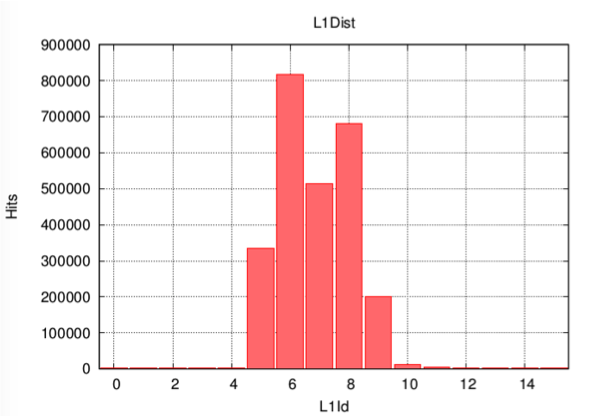
\includegraphics[width=8cm]{./figure/l1dist.png}
  \caption{アナログスキャンの時のL1IDの分布}
  \label{fig:YARRDAQ}
\end{figure}

理想的にはL1IDが7のところにトリガの中心を合わせたい.そのために,YARRで指定できるLatencyに関する2種類のパラメータを以下に示す.

%\subsubsection*{ソフトウェアで設定されている''delay''}
%擬似パルスを送られてからどれくらい遅れてトリガを出力するかを決める値.前章で述べたデジタルスキャンやアナログスキャンの際に関係し,擬似パルスではなく外部からのトリガを使用してデータ取得するセルフトリガや外部トリガを用いたデータ取得の時には無関係.
%

\subsubsection*{a. ファームウェアの設定値''delay''}
図\ref{fig:YARRDAQ}のaで示されている部分.FPGAからトリガをどれだけ遅れて出力するかを決める値.本論文では,外部からトリガを受け取ってからどれくらい遅延させてFPGAからRD53Aにトリガを出力するかを決める値.

\subsubsection*{b. グローバルレジスタ''LatencyConfig''}
RD53Aの全てのピクセルに共通する設定値であるグローバルレジスタの内の1つにLatencyConfigというLatencyに関する設定値が存在する.LatencyConfigがどのような値であるか説明する図を以下に示す.\par
ASICのあるピクセルが信号を検知すると,そのピクセルが40 $\mathrm{MHz}$のClockに合わせてカウントを始める.そして,FPGAから送られてくるトリガを受け取った時に,そのカウントが設定した''LatencyConfig''の値と等しいピクセルの情報を読み出すようになっている.''LatencyConfig''は,9bitの値であり,0-511まで変化させることが可能である.

\subsection{Latency Scan機能}
前節で述べたように,Latencyが合っていないと,データを正しく読み出すことができないので,Latencyを正しい値にすることが,データを正しく読み出す上で大変重要となる.そこで,今回はグローバルレジスタ''LatencyConfig''値を変化させることで,Latencyを合わせられるような機能をYARRに追加した.\par
今回,センサからの信号をASICがHitOR信号として出力したTriggerに対するLatencyを合わせたかった.前章で述べたように,HitOR信号がFPGAに伝わっていることを確認した上で,以下を行なった.
\begin{enumerate}
\item セルフトリガによって100イベントを取得する
\item 取得したデータのL1IDの分布を得る
\item $\mathrm{L1ID} == 7$であるイベント数を記録
\end{enumerate}
以上を0-511の各''LatencyConfig''値に対して行い,''LatencyConfig''値と$\mathrm{L1ID} == 7$だったイベント数の関係を図\ref{fig:latencydist}のように得る.,この時にもっともイベント数が多かった''LatencyConfig''値の時にLatencyが合っていると定義した,

\begin{figure}[h]
  \centering
  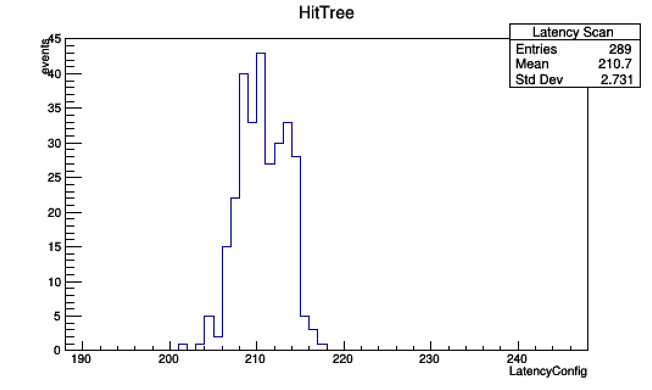
\includegraphics[width=14cm]{./figure/latencydist.png}
  \caption{''LatencyConfig''値とL1ID $== 7$だったイベント数の関係}
  \label{fig:latencydist}
\end{figure}


\subsubsection*{Latencyチューニングが幅を持つ理由}
理想的には,Latency Scanを行なった時の分布は,正しいLatency値にのみピークが立つはずであるが,今回の結果はそうはなっていない.理由は2つある.

\begin{itemize}
\item YARRのファームウェアの仕組みとして,RD53Aに向けて出力されるコマンドは160 $\mathrm{MHz}$のClockで32 $\mathrm{bit}$単位で送る必要がある.しかし,RD53AはLHCのバンチ衝突のレートである40 $\mathrm{MHz}$でヒットが生成されることを前提に設計されている.したがって,8BC分のトリガをまとめてファームウェアから出力する必要があるのだが,YARRのファームウェアの仕組みとして,そのタイミングを正確に合わせていないため,前後8 BC分の幅が生じてしまう.\\
  
%\item YARRの仕組みとして,32bitに1回トリガを発行するかどうかを決めているので,前後8 $\mathrm{Clock}$分の幅が生じる
\item 図\ref{fig:analogop}はDiff FEのアナログ回路の先を示しており,図\ref{fig:DiffFE}の一番右のCompの部分が図\ref{fig:analogop}の一番左のCompに対応する.アナログ回路から出力された信号はフリップフロップ回路に入力される.しかし,その間に寄生容量(図中の\ref{fig:analogop}の$C_p$)が生じているため,出力のタイミングに前後2 BCの幅が生じてしまう.これがLatency SCanの結果にも影響する.


    %\item アナログアウトプットのキャパシタンスにズレがあるために前後2 $\mathrm{Clock}$分の幅が生じる.これは,アナログスキャンを行なった時のL1IDの分布を見ると,$\mathrm{L1ID} == 7$のところにのみピークが立つのではなく,前後に2 $\mathrm{Clock}$分の幅を持っていることから確認できる.
\end{itemize}

\begin{figure}[h]
  \centering
  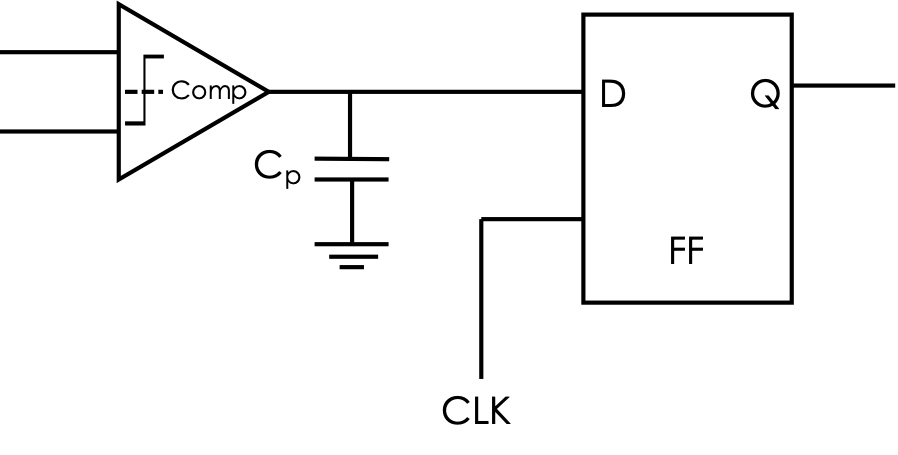
\includegraphics[width=8cm]{./figure/analogop.png}
  \caption{Diff FEのアナログ回路の出力}
  \label{fig:analogop}
\end{figure}


\section{セルフトリガを用いた応答試験セットアップ}
\label{sec:selfsetup}
主なセットアップは読み出しシステムの動作確認時の図\ref{fig:setup}と変わらず,RD53A搭載のSingle Chip Card(SCC)とFPGAボード,PCを用いて読み出しシステムを構成し,SCCとFPGAボードはアダプタカードを用いてディスプレイポートケーブルによって接続した.センサからの信号を外部に出力するためのコネクタをアダプタカードのport D,FPGAがRD53Aからのデータを受け取るためのコネクタをアダプタカードのport Aに繋ぐようにしている.

\section{セルフトリガによるデータ取得手順}
\label{sec:selfhow}
前章で述べたHitOR信号の伝達確認を行なったのち,前節で述べたLatencyチューニングをセンサの上に線源を配置してから行った.''LatencyConfig''の分布が図\ref{fig:latencydist}のように得られたため,今回は''LatencyConfig''の値を211に設定することで,Latencyを合わせた.Latencyを合わせた上で,以下の3つのトリガ生成方法でデータ取得を行う.
\begin{enumerate}
\item 200 $\mathrm{kHz}$でトリガを生成し,データ取得を行う
\item 線源を置かない状態でセルフトリガによるデータ取得を行う
\item 線源を置いた状態でセルフトリガによるデータ取得を行う
\end{enumerate}

%応答評価試験として,センサの上に線源を置いて30分間のセルフトリガによるデータ取得を行なった.また,背景事象の測定として,30分間線源を置かずにセルフトリガによるデータ取得を行なった.

\section{セルフトリガによるデータ取得結果}
\label{sec:selfconc}
3つのトリガ生成方法で得られたデータのトリガ数とヒット数を表\ref{tab:self}に示す.

\begin{table}[h]
  \centering
  \caption{トリガ生成方法に対する得られたヒット数とトリガ数}
  \begin{tabular} {l|ccc} \hline
    トリガ生成方法 & ランダムトリガ & セルフトリガ(線源なし) & セルフトリガ(線源あり) \\ \hline
    ヒット数 & & & 3599457 \\
    トリガ数 & $6 \time 10^6$ & 4193685 & 4056311 \\ \hline
  \end{tabular}
  \label{tab:selfpara}
\end{table}

\section{考察}

\subsection*{トリガ生成方法と取得されるデータの内容}
3つのトリガ生成方法による取得されるデータの内容の違いについて表\ref{tab:selfdata}に示す.

\begin{table}[h]
  \centering
  \caption{トリガ生成方法と取得されるデータの内容}
  \begin{tabular} {l|ccc} \hline
    & ランダムトリガ & セルフトリガ(線源なし) & セルフトリガ(線源あり) \\ \hline
    トリガ生成方法 & 200 $\mathrm{kHz}$のトリガ & センサの信号でトリガ生成 & センサからの信号でトリガ生成 \\ \hline
    取得される & 無関係なトリガで & 無関係なトリガで & 無関係なトリガで\\
    データの内容 & 得られるヒット & 得られるヒット & 得られるヒット \\
    & & センサのノイズ & センサのノイズ \\
    & & & 荷電粒子の信号\\ \hline
  \end{tabular}
  \label{tab:selfdata}
\end{table}

よって,線源ありのセルフトリガによって取得されたデータから,無関係なトリガで得られるヒットと,センサのノイズによる影響を除くことで,荷電粒子からの信号を見積りたい.

\subsection*{荷電粒子からの信号の見積もり}
荷電粒子からの信号を見積もるために,各ピクセルが得たヒット数に着目する.i番目のピクセルに対して,表\ref{tab:selfpara}のように値を定める.
  \begin{table}[h]
    \centering
    \caption{i番目のピクセルに対して得られる値}
    \begin{tabular} {l|ccc} \hline
      & ランダムトリガ & セルフトリガ(線源なし) & セルフトリガ(線源あり) \\ \hline
      ヒット数 & $N_{\mathrm{i.bg}}^{\mathrm{random}}$& $N_{\mathrm{i.bg}}^{\mathrm{self}}$ & $N_{\mathrm{i}}^{\mathrm{self}}$ \\
      トリガ数 & $M_{\mathrm{i.bg}}^{\mathrm{random}}$ & $M_{\mathrm{i}}^{\mathrm{self}}$ \\
      トリガ数に対するヒット数 & $N_{\mathrm{i.bg}}^{\mathrm{random}}$ & $R_{\mathrm{i.bg}}^{\mathrm{self}}$ & $R_{\mathrm{i}}^{\mathrm{self}}$ \\\hline
    \end{tabular}
    \label{tab:selfpara}
  \end{table}


この時,$N_{\mathrm{i}}^{\mathrm{self}}$に対して,ランダムトリガによる影響を除いたもの$N_{\mathrm{i.sig'}}$と,それに加えてセンサノイズによる影響を除いた$N_{\mathrm{i.sig}}$を式\ref{eq:selfphits}のように表す.$N_{\mathrm{i.sig}}$が荷電粒子による信号の見積もりである.
  
\begin{eqnarray}
  \label{eq:selfphits1}
  N_{\mathrm{i.sig'}} &=& N_{\mathrm{i}} - \mathrm{i.Random} \\
  \mathrm{i.Random} &=& \frac{N_{\mathrm{i.bg}}^{\mathrm{random}}}{M_{\mathrm{i.bg}}^{\mathrm{random}}} \times M_{\mathrm{i}}^{\mathrm{self}}\\
  N_{\mathrm{i.sig}} &=& N_{\mathrm{i}} - \mathrm{i.Background} \\
  \mathrm{i.Background} &=& \left(\frac{N_{\mathrm{i.bg}}^{\mathrm{self}}}{M_{\mathrm{i.bg}}^{\mathrm{self}}} + \frac{N_{\mathrm{i.bg}}^{\mathrm{random}}}{M_{\mathrm{i.bg}}^{\mathrm{random}}} \right) \times M_{\mathrm{i}}^{\mathrm{self}}
\end{eqnarray}

$N_{\mathrm{i}}$と$N_{\mathrm{i.sig'}}$1ピクセルあたりのヒット数分布の違いを図\ref{fig:selfhitsperpix1}に示す.
\begin{figure}[h]
  \centering
  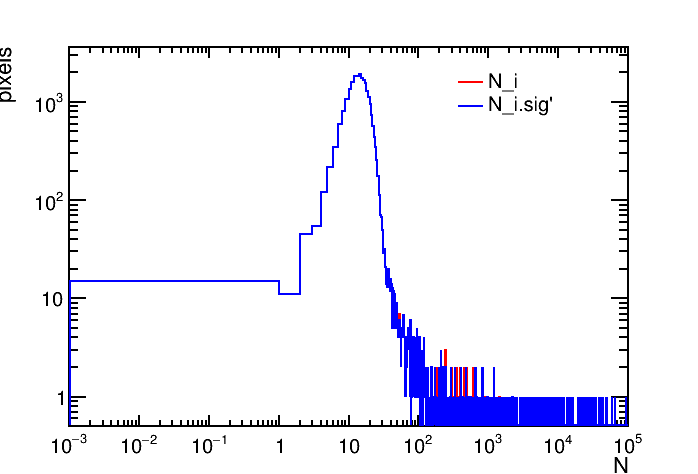
\includegraphics[width=10cm]{./figure/selfhitperpix1.png}
  \caption{1ピクセルあたりのHit数分布}
  \label{fig:selfhitfreq}
\end{figure}

$N_{\mathrm{i}}$と$N_{\mathrm{i.sig'}}$1ピクセルあたりのヒット数分布の推移を図\ref{fig:selfhitsperpix1bfaf}に示す.横軸が$N_{\mathrm{i}}$で縦軸が$N_{\mathrm{i.sig}}$を示していて,分布はほぼ線形であり,補正前後で分布に変化がなく,$N_{\mathrm{i}}$の分布にランダムトリガによる影響はほとんどないことがわかる.
\begin{figure}[h]
  \centering
  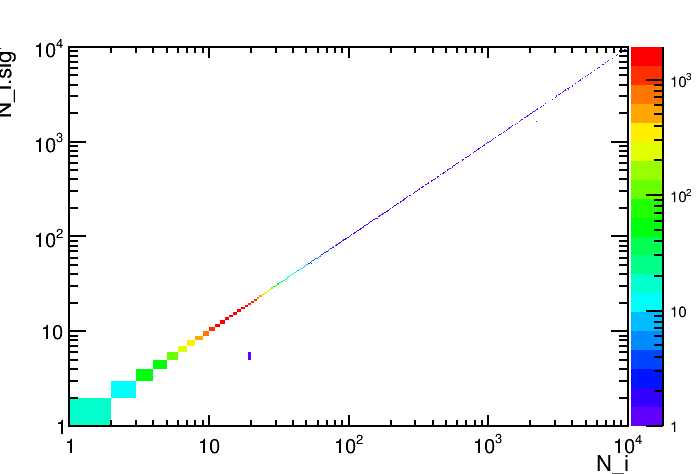
\includegraphics[width=10cm]{./figure/selfhitperpixbfaf1.png}
  \caption{1ピクセルあたりのHit数分布}
  \label{fig:selfhitfreq}
\end{figure}

次に,$N_{\mathrm{i}}$と$N_{\mathrm{i.sig'}}$1ピクセルあたりのヒット数分布の違いを図\ref{fig:selfhitsperpix1}に示す.
\begin{figure}[h]
  \centering
  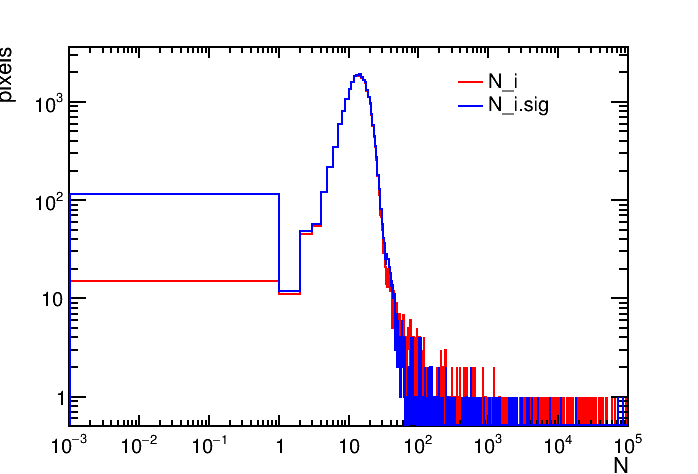
\includegraphics[width=10cm]{./figure/selfhitperpix.png}
  \caption{1ピクセルあたりのHit数分布}
  \label{fig:selfhitfreq}
\end{figure}

$N_{\mathrm{i}}$と$N_{\mathrm{i.sig'}}$1ピクセルあたりのヒット数分布の推移を図\ref{fig:selfhitsperpix1bfaf}に示す.横軸が$N_{\mathrm{i}}$で縦軸が$N_{\mathrm{i.sig}}$を示していて,$N_{\mathrm{i}}$が10 $\mathrm{Hits}$以下の部分は線形であるのに対し,$N_{\mathrm{i}}$の値が大きい分布は$N_{\mathrm{i.sig}}$では0に分布しているものが多く,センサノイズの影響が大きいことがわかる.
\begin{figure}[h]
  \centering
  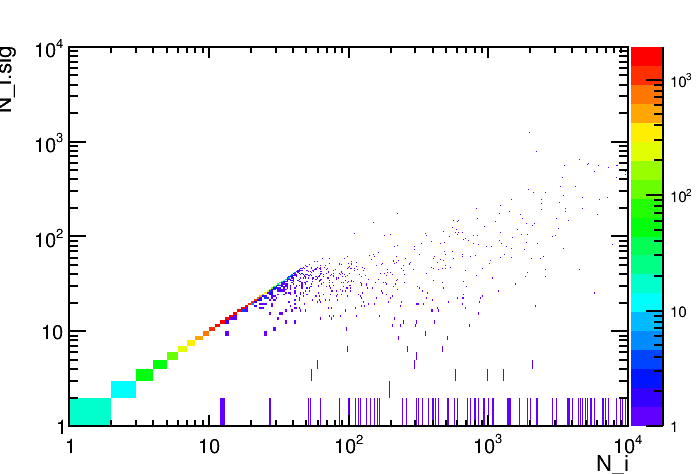
\includegraphics[width=10cm]{./figure/selfhitperpixbfaf.png}
  \caption{1ピクセルあたりのHit数分布}
  \label{fig:selfhitfreq}
\end{figure}

最終的に得られた荷電粒子の信号$N_{\mathrm{i.sig}}$の分布はポアソン分布式\ref{eq:poisson}に従うので,フィッティングを行い,平均ヒット数を求めた.フィッティングを行なった様子を図\ref{fig:selffit}に示す.

\begin{eqnarray}
  \label{eq:poisson}
  P(x) = \frac{\lambda^x e^{-\lambda}}{x!} (\lambda:\mathrm{const})
\end{eqnarray}

\begin{figure}[h]
  \centering
  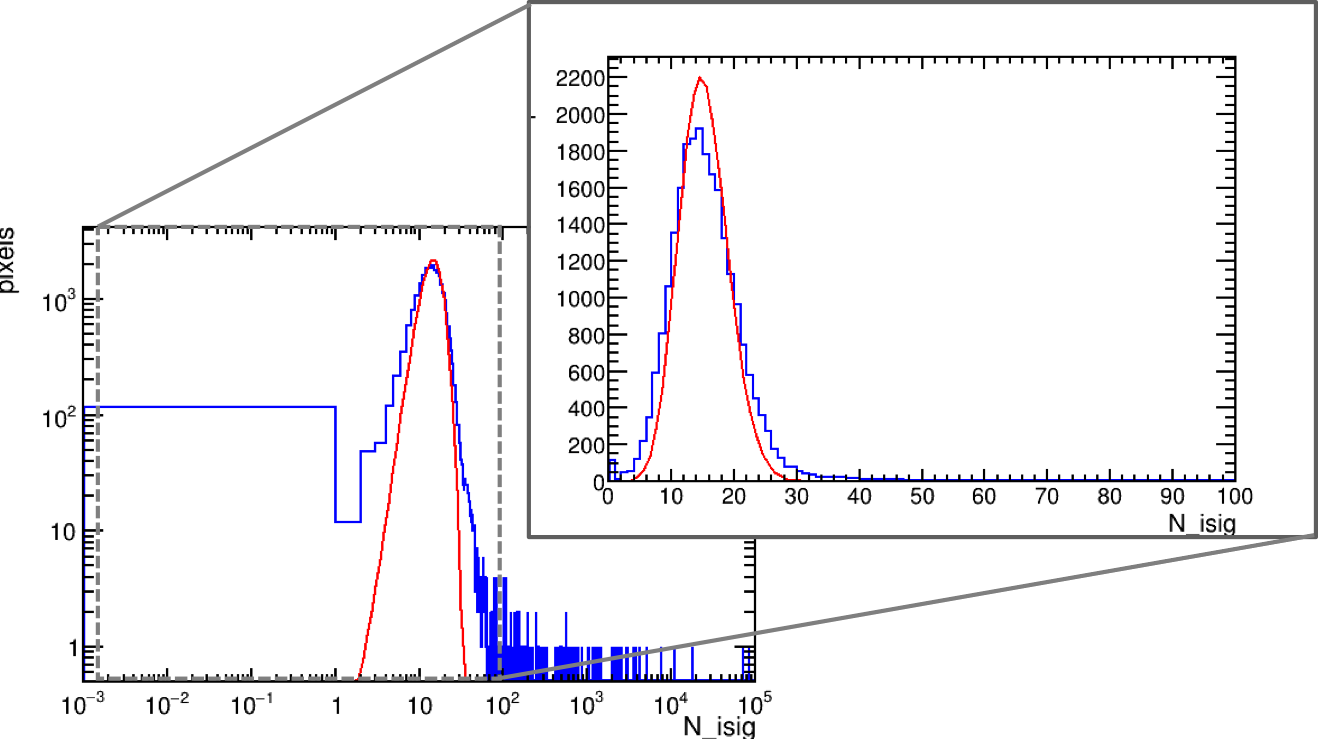
\includegraphics[width=15cm]{./figure/selffit.png}
  \caption{1ピクセルあたりのHit数分布}
  \label{fig:selfhitfreq}
\end{figure}

フィットの結果より,30分のセルフトリガによる応答評価試験で得られる1ピクセルあたりの平均ヒット数は15.1 $\mathrm{Hits/pixel}$と求められた.品質評価に必要なヒット数50 $\mathrm{Hits/pixel}$を得るためには,およそ100分かかることがわかった.

\subsection*{全ヒット数に対する荷電粒子によるヒット数}
全ヒット数$N$と,背景事象によるヒット数$N_{\mathrm{bg}}$,荷電粒子によるヒット数$N_{\mathrm{sig}}$の定義を式\ref{eq:selfallhits}に示す.

\begin{eqnarray}
  N &=& \sum^{\mathrm{allpixels}} N_{\mathrm{i}} \\
  N_{\mathrm{bg}} &=& \sum^{\mathrm{allpixels}} \left(N_{\mathrm{i.bg}}^{\mathrm{random}} + N_{\mathrm{i.bg}}^{\mathrm{self}} \right) \\
  N_{\mathrm{sig}} &=& \sum^{\mathrm{allpixels}} N_{\mathrm{i.sig}}
\end{eqnarray}

セルフトリガによる応答評価試験で得られた$N$に対する$N_{\mathrm{sig}}$の割合とヒットレートを表\ref{tab:selfp}に示す.
\begin{table}[h]
  \centering
  \caption{30分間で得られた荷電粒子のヒット数}
  \begin{tabular} {l|ccc} \hline
    time:1800[sec]& $N$ & $N_{\mathrm{bg}}$ & $N_{\mathrm{sig}}$ \\ \hline
    ヒット数 & 3599457 & 2954185 & 645272 \\
    & (100 \%) & (82.1 \%) & (17.9 \%) \\ \hline
    ヒット数/time & 1999.7 $\mathrm{Hz}$ & 1641.2 $\mathrm{Hz}$ & 358.5 $\mathrm{Hz}$ \\ \hline
  \end{tabular}
  \label{tab:selfp}
\end{table}

荷電粒子によるヒットレート(ヒット数/time)は358.5 $\mathrm{Hz}$と高い結果になっているが,$N$に対する$N_{\mathrm{i.sig}}$の割合は17.9 \%と低い結果となった.

\subsection*{ヒット情報をもつイベント数}
全トリガ数$M$に対する,ヒットが存在しなかったイベント数$M_{\mathrm{emp}}$と,存在したイベント数$M_{\mathrm{data}}$の割合とトリガレートを表\ref{tab:selfr}に示す.

\begin{table}[h]
  \centering
  \caption{全トリガ数と対するヒットが存在したイベント数の割合}
  \begin{tabular} {l|ccc} \hline
    time:1800[sec] & $M$ & $M_{\mathrm{data}}$ & $M_{\mathrm{emp}}$ \\ \hline
    トリガ数 & 4056311 & 3528141 & 528170 \\
     & (100 \%) & (87.0 \%) & (13.0 \%) \\ \hline
    トリガ数/time & 2254 $\mathrm{Hz}$ & 1960 $\mathrm{Hz}$ & 293.4 $\mathrm{Hz}$ \\ \hline
  \end{tabular}
  \label{tab:selfr}
\end{table}

$M$に対する$M_{\mathrm{data}}$の割合は87.0 \%と,ほとんどのトリガに対して,ヒットのデータが取得できていることがわかった.

